\section{Architectural Failure Effect Modeling for the WBS}

We illustrate our FEM approach on the Wheel Braking System.  Starting from the nominal model described in Section~\ref{sec:nominal}, we first determine whether a given safety property of interest holds on a fault-free instance of the model.  We then extend the model with faults and determine whether the property continues to hold under reasonable fault scenarios.

The initial safety property to be proven determines whether the system will apply pressure to the wheels when commanded to do so: 

\begin{tt} 
\  \\ 
If pedals are pressed and no skid occurs, then the brakes will receive pressure. \\
\end{tt}

\noindent Using the reference AADL model constructed by the SEI~\cite{SEI:AADL} extended with AGREE contracts describing system behaviors, this property proves immediately.  From this point, we focus our attention on component failures and how this will affect the top level property of the system.

We would like to specify different component failure modes. These failure modes can be triggered by some internal error or a propagated fault. In order to trigger these faults, additional input was added to the AADL model for each fault that can occur within a nominal model component. Our initial fault model consists of two fault types:

\begin{itemize}
\item \textit{fail\_to} fault: This type of fault accounts for both nondeterministic failures and stuck-at failures. The components that are affected by this fault include meter valves and pumps. This fault can be used to describe both digital and mechanical errors. Examples of digital errors include a \textit{stuck\_at} failure for the Command subsystem in the BSCU component, which causes the Command unit to become stuck at a previous value. An example of a mechanical error would be a valve stuck open (or closed). 

%%%%%%% DANIELLE
%                     CHECK INTO MECHANICAL FAILURES

\item \textit{inverted\_fail} fault: This type of fault will be used on components which contain boolean output. It will simply take boolean input, negate it, and output the negated value. An example of this is the Selector. In the nominal model, input to the Selector consists of a boolean value \textit{select\_alternate} value from the BSCU. This value determines the switch of the system from Normal pressure to Alternate pressure. If this value is inverted, the pressure will not be selected according to the requirement description.  

\end{itemize}

\begin{figure}[h!]
  \centering
 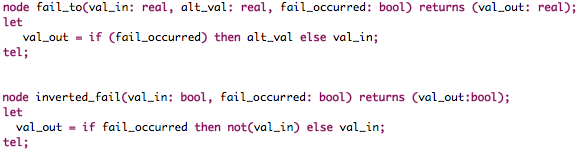
\includegraphics[width=1\textwidth]{images/failureNodes.png}
  \vspace{-0.1in}
  \caption{AGREE Definition of a \textit{fail\_to} and \textit{inverted\_failure} Faults}
  \label{fig:failureNodes}
\end{figure}

These faults can be easily encoded in AGREE as shown in Figure~\ref{fig:failureNodes}.  The failures simply return an alternate value (for {\em fail\_to}) or invert the input value (for {\em inverted\_failure}) when a failure occurs.
 

While modeling faults, the duration of the fault must also be taken into account.  The AGREE tools allow a great deal of flexibility in terms of how faults are defined and their duration.  For the purposes of this model, we currently consider only {\em transient} and {\em permanent} faults, where transient faults occur for an instant in time (e.g., a single-event upset) and a permanent fault persists for the remainder of the system execution.


\subsection{Analysis of Faulty Models}
The following is a short summary of the failures defined in the fault model.

\begin{itemize}

\item Valves and Pumps: All valves and pumps have the possibility of a \textit{fail\_to} fault. This includes Green pump, Blue pump, Accumulator, and the Shutoff valves.

\item  The Selector can also have a digital \textit{fail\_to} fault regarding the inputs from BSCU commanding to use Normal or Alternate means of pressure along with an \textit{inverted\_fail} fault which would change the boolean value that commands antiskid to activate.

\end{itemize}

Given our understanding of the WBS, our assumption was that any single permanent fault could be introduced into the system and the pilot would still be able to command brake pressure.  However, our analysis tools returned a counterexample to the property, and upon examination, the structure of the reference model was insufficient to guarantee the property.  

%\subsection{Strengthening the Nominal Model}
The first issue that was discovered involved {\em feedback}; the reference model did not have a sensor to determine pressure after the selector valve.  This means that a single failure of (for example) the blue or green antiskid valve cannot be detected by the BSCU (see Figure~\ref{fig:wbs_ima}), and so it cannot route around the failure.  In order to fix this, we added a pressure sensor to the wheel that communicates with the BSCU to detect lack of pressure at the wheel.


After adding a sensing apparatus to the wheel, the analysis generated another counterexample due to a single failure of the selector valve.  In the reference model, there is a single selector component that takes as inputs the Green Pump, the Blue Pump, and the Accumulator.  A single failure in this component can lead to no pressure along either of the two outgoing pressure lines.
To solve this issue, we removed the accumulator from the selector and added an accumulator valve.   This component takes in the Blue pressure from the Selector and the Accumulator pressure. It also takes in a \textit{select\_alternate} flag from the BSCU. The output of the Accumulator\_Valve goes directly to the Blue\_Skid component and is either the blue or the accumulator pressure.

Finally, our BSCU is currently structured to always fail-over from the Green system to the Blue system but never the reverse.  Because of this choice (which matches the ARP document), it is also necessary to guarantee that \textit{select\_alternate} is false until a failure occurs in the system; otherwise, a single failure in the blue anti-skid valve can cause the system to fail to provide pressure.  This assymetry is something that could be revisited in future work.


Even after making these three fixes to the model, the original property still does not prove.  At issue is that the sensing of a no-pressure situation is not instantaneous; there is a delay for this information to reach the BSCU and be acted upon to switch to the alternate braking system.  In our current timing model for the system, the feedback to the BSCU involves a cycle delay, but the BSCU and valves can react instantaneously.  Thus, we weaken our top-level property to state that if the brakes are pressed for two consecutive time instants, then pressure will be provided to the wheels:

\begin{tt}
\ \\ 
If pedals are pressed in the previous state and pressed in the current state and no skid occurs, then the brakes will receive pressure. \\ 
\end{tt}


















